\section{Описание алгоритма}
Весь процесс построения выпуклой оболочки для компонент бинарного изображения можно разделить на \textbf{2 этапа}:
\begin{enumerate}
	\item выделение компонент бинарного изображения;
	\item построение выпуклой оболочки.
\end{enumerate}
\subsection{Выделение компонент бинарного изображения}
На данном этапе каждому пикселю каждой компоненты присваивается номер. Тем самым происходит идентификация каждой компоненты, то есть отделение их друг от друга.\n
В данной лабораторной работе процесс выделения компонент реализован с помощью циклического алгоритма, использующего очередь задач.
\subsection{Построение выпуклой оболочки}
После завершения первого этапа образуется набор компонент. Однако изображение чаще всего имеет достаточно плотную структуру, поэтому в целях оптимизации компоненты дополнительно приводятся к более простому виду. Из рассмотрения удаляются точки, которые имеют более двух ненулевых соседей, а также те, которые имеют двух ненулевых соседей на одной линии (справа и слева или сверху и снизу от текущего пикселя). Данная процедура позволяет уменьшить количество рассматриваемых точек до минимума.\n
Для построения выпуклой оболочки для каждой компоненты бинарного изображения был выбран алгоритма Грэхема. На вход данному алгоритму подается массив точек, которые принадлежат конкретной компоненте.\n
Работу данного алгоритма можно разделить на несколько \textbf{этапов}:
\begin{enumerate}
	\item выбираем точку из массива с минимальной $x$-координатой (если таких несколько, берем самую верхнюю из них), добавляем ее в ответ;
	\item упорядочиваем оставшиеся точки по углу, который они образуют с выбранной точкой;
	\item добавляем в ответ $p_1$ - первую точку из упорядоченного списка;
	\item берем следующую точку $k$, и пока $k$ и две предыдущие точки в текущей оболочке ($p_i$ и $p_{i−1}$) образуют векторы ($p_i$$k$ и $p_i$$p_{i−1}$), которые лежат не по часовой стрелке, исключаем из оболочки $p_i$;
	\item добавляем в оболочку точку $k$;
	\item повторяем пункты 4-5, пока есть точки.
\end{enumerate}
\begin{figure}[H]
	\centering
	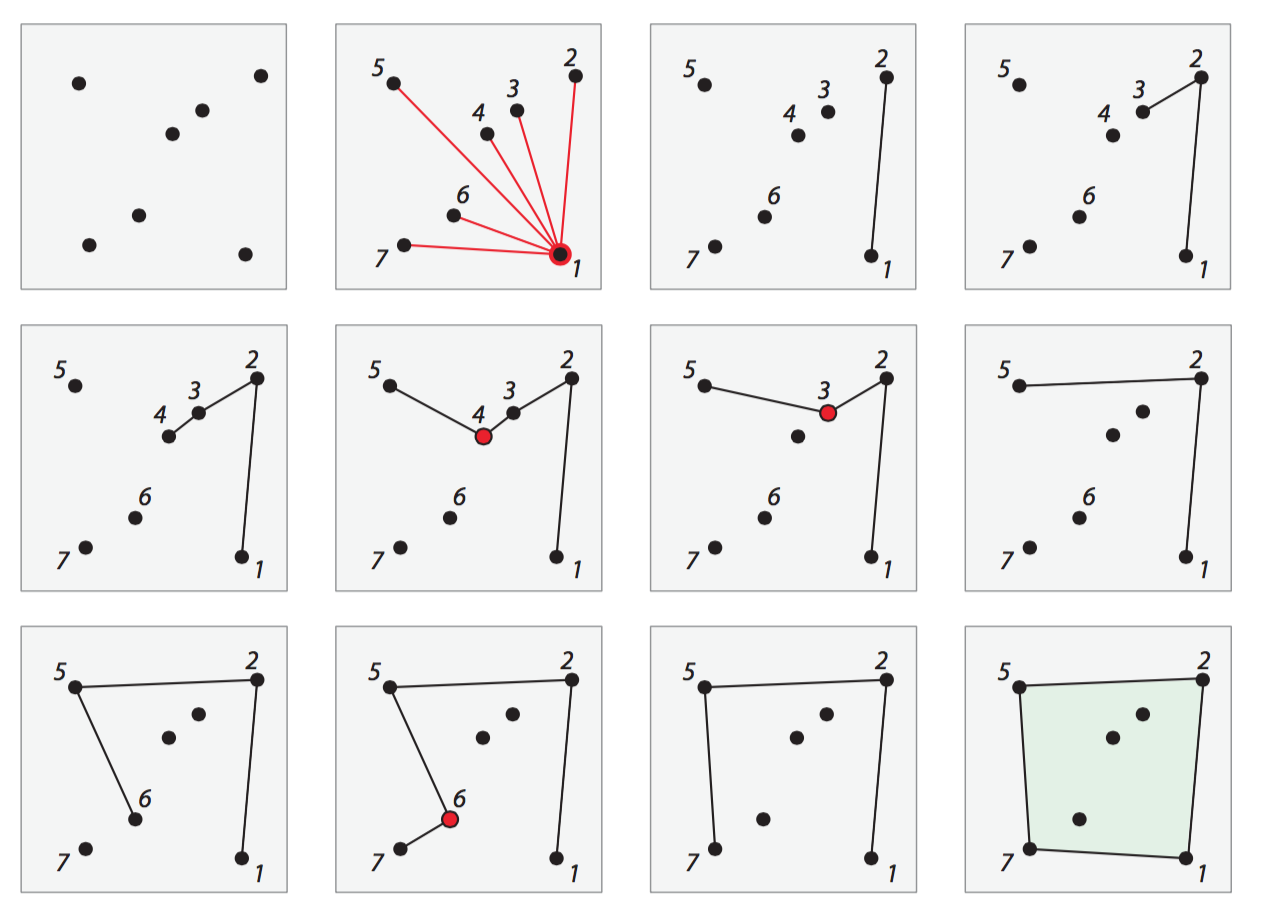
\includegraphics[width=\linewidth]{img/graham}
	\caption{Алгоритм Грэхема в действии. Красные точки образуют левый поворот и удаляются из оболочки.}
	\label{fig:graham}
\end{figure}
